% !TeX program = LuaLaTeX
\documentclass[aspectratio=169, 10pt]{beamer}\usepackage[]{graphicx}\usepackage[]{xcolor}
% maxwidth is the original width if it is less than linewidth
% otherwise use linewidth (to make sure the graphics do not exceed the margin)
\makeatletter
\def\maxwidth{ %
  \ifdim\Gin@nat@width>\linewidth
    \linewidth
  \else
    \Gin@nat@width
  \fi
}
\makeatother

\definecolor{fgcolor}{rgb}{0.345, 0.345, 0.345}
\newcommand{\hlnum}[1]{\textcolor[rgb]{0.686,0.059,0.569}{#1}}%
\newcommand{\hlsng}[1]{\textcolor[rgb]{0.192,0.494,0.8}{#1}}%
\newcommand{\hlcom}[1]{\textcolor[rgb]{0.678,0.584,0.686}{\textit{#1}}}%
\newcommand{\hlopt}[1]{\textcolor[rgb]{0,0,0}{#1}}%
\newcommand{\hldef}[1]{\textcolor[rgb]{0.345,0.345,0.345}{#1}}%
\newcommand{\hlkwa}[1]{\textcolor[rgb]{0.161,0.373,0.58}{\textbf{#1}}}%
\newcommand{\hlkwb}[1]{\textcolor[rgb]{0.69,0.353,0.396}{#1}}%
\newcommand{\hlkwc}[1]{\textcolor[rgb]{0.333,0.667,0.333}{#1}}%
\newcommand{\hlkwd}[1]{\textcolor[rgb]{0.737,0.353,0.396}{\textbf{#1}}}%
\let\hlipl\hlkwb

\usepackage{framed}
\makeatletter
\newenvironment{kframe}{%
 \def\at@end@of@kframe{}%
 \ifinner\ifhmode%
  \def\at@end@of@kframe{\end{minipage}}%
  \begin{minipage}{\columnwidth}%
 \fi\fi%
 \def\FrameCommand##1{\hskip\@totalleftmargin \hskip-\fboxsep
 \colorbox{shadecolor}{##1}\hskip-\fboxsep
     % There is no \\@totalrightmargin, so:
     \hskip-\linewidth \hskip-\@totalleftmargin \hskip\columnwidth}%
 \MakeFramed {\advance\hsize-\width
   \@totalleftmargin\z@ \linewidth\hsize
   \@setminipage}}%
 {\par\unskip\endMakeFramed%
 \at@end@of@kframe}
\makeatother

\definecolor{shadecolor}{rgb}{.97, .97, .97}
\definecolor{messagecolor}{rgb}{0, 0, 0}
\definecolor{warningcolor}{rgb}{1, 0, 1}
\definecolor{errorcolor}{rgb}{1, 0, 0}
\newenvironment{knitrout}{}{} % an empty environment to be redefined in TeX

\usepackage{alltt}
\usetheme{gotham}
% % \newcommand\seq[2]{{#1}\!:\!{#2}}
\newcommand\seq[2]{{#1}:{#2}}
\def\lik{L}
\def\loglik{\ell}
\newcommand\R{\mathbb{R}}
\newcommand\paramVec{\theta}
\newcommand\myeqref[1]{(\ref{#1})}
\newcommand\MApar{\varphi}
\newcommand\code[1]{\texttt{#1}}


	\gothamset{
		numbering=totalframenumber,
		% tocframe template= gotham simple,
		% progressbar position=circlehead,
		progressbar position=foot,
		progressbar style=rectangle,
		progressbar mfn=on,
		parttocframe default=off,
		sectiontocframe default=off,
		subsectiontocframe default=off,
		title page=gotham normal,
	}

	\usepackage{standalone}
	\usepackage{colortbl,xcolor}
	\usepackage{natbib}
	\usepackage{tikz}
	\usepackage{bm}
	\usepackage{mathtools}
	\usepackage{pgfplots}
	\usepackage{tabularray} % Typeset tabulars and arrays (contains equivalent of longtable, booktabs and dcolumn at least) 
		\UseTblrLibrary{booktabs} % to load extra commands from booktabs
	\usepackage{changepage}
	\usepackage{appendixnumberbeamer}
		\newcommand{\famName}[1]{\textsc{#1}}
	\usepackage{minted}
		\definecolor{codeback}{rgb}{0.90,0.91,0.92}
		\definecolor{codebackdark}{rgb}{0.10,0.11,0.12}
		\usemintedstyle{emacs}
		\setmintedinline[tex]{bgcolor=codeback}
		\setminted[tex]{
			autogobble,
			bgcolor=codeback,
			tabsize=4,
			extrakeywords={usetheme,institute,maketitle,subtitle,gothamset,colorlet,setbeamercolor,plain,defbeamertemplate}
		}

	\usepackage[scale=2]{ccicons}
	% \usepackage{pgfplots}
		\usepgfplotslibrary{dateplot}

	\newcommand{\themename}{\textbf{\textsc{Gotham}}}

% \renewcommand{\gothamInstituteLogoSquare}[1][4 ex]{
% 
\includegraphics[height=#1]{michiganM.png}
% }

\setbeamercolor{block title}{bg=colorA!70!gray}
% \setbeamercolor{block body}{bg=colorA!20!white}
\setbeamercolor{block body}{
use={block title},
bg=block title.bg!20!white
}

\title[]{Innovations in Likelihood-Based Inference for State Space Models}
\subtitle{Oral Defense}
\date[May 2025]{\today}
\author[Wheeler, J.]{Jesse Wheeler}
\institute{Department of Statistics, University of Michigan}
% \titlegraphic{\hfill
\includegraphics[height=1.5cm]{michiganM.png}}
\renewcommand{\gothamtitlepagelogo}{%
  \hfill
\includegraphics[height=1.5cm]{michiganM.png}\hspace{-1.4cm}
}
\renewcommand{\gothamInstituteLogoSquare}[1][3ex]{%
		
\includegraphics[height=#1]{michiganM.png}
}
% \titlegraphic{\hfill
\includegraphics[height=1.5cm]{gotham-logo.pdf}}

% \newcommand\seq[2]{{#1}\!:\!{#2}}
\newcommand\seq[2]{{#1}:{#2}}
\def\lik{L}
\def\loglik{\ell}
\newcommand\R{\mathbb{R}}
\newcommand\paramVec{\theta}
\newcommand\myeqref[1]{(\ref{#1})}
\newcommand\MApar{\varphi}
\newcommand\code[1]{\texttt{#1}}


\makeatletter
% \newcommand\notsotiny{\@setfontsize\notsotiny\@vipt\@viipt}
\newcommand\notsotiny{\@setfontsize\notsotiny{6.6}{7.3}}
\makeatother
\IfFileExists{upquote.sty}{\usepackage{upquote}}{}
\begin{document}


\maketitle

	\begin{frame}[toc]{Table of contents}%
		\tableofcontents%[hideallsubsections]
	\end{frame}

	
%%%%%%%%%%%%%%%%%%%%
%%%  MAINMATTER  %%%
%%%%%%%%%%%%%%%%%%%%
% \documentclass[aspectratio=169]{beamer}

	\usepackage{standalone}
	\usepackage{tikz}
	\usepackage{pgfplots}

	\usepackage{tabularray} % Typeset tabulars and arrays (contains equivalent of longtable, booktabs and dcolumn at least) 
		\UseTblrLibrary{booktabs} % to load extra commands from booktabs

	\usepackage{natbib}
\begin{filecontents*}[overwrite]{pres.bib}
@article{Knuth92,
	author = "D.E. Knuth",
	title = "Two notes on notation",
	journal = "Amer. Math. Monthly",
	volume = "99",
	year = "1992",
	pages = "403--422",
}

@book{ConcreteMath,
	author = "R.L. Graham and D.E. Knuth and O. Patashnik",
	title = "Concrete mathematics",
	publisher = "Addison-Wesley",
	address = "Reading, MA",
	year = "1989"
}

@unpublished{Simpson,
	author = "H. Simpson",
	title = "Proof of the {R}iemann {H}ypothesis",
	note = "preprint (2003), available at \texttt{http://www.math.drofnats.edu/riemann.ps}",
	year = "2003"
}

@incollection{Er01,
	author = "P. Erd{\H o}s",
	title = "A selection of problems and results in combinatorics",
	booktitle = "Recent trends in combinatorics (Matrahaza, 1995)",
	publisher = "Cambridge Univ. Press",
	address = "Cambridge",
	pages = "1--6",
	year = "1995"
}

@article{greenwade93,
	author  = "George D. Greenwade",
	title   = "The {C}omprehensive {T}ex {A}rchive {N}etwork ({CTAN})",
	year    = "1993",
	journal = "TUGBoat",
	volume  = "14",
	number  = "3",
	pages   = "342--351"
}
\end{filecontents*}


\begin{document}

\section{Introduction: Beamer}

	% FRAME
	\begin{frame}[fragile]{Title page}
		The Title page is printed using the command:			
		\begin{verbatim}    \maketitle\end{verbatim}
		
		The element printed on this page are defined in the preamble by
		\begin{verbatim}
			\title[]{Gotham}
			\subtitle{A Modern, versatile and extendable theme for Beamer}
			\date[]{\today}
			\author[]{Romain NOËL}
			\institute{Center for modern beamer themes}
			% \titlegraphic{\hfill\includegraphics[height=1.5cm, draft]{Title_logo.pdf}}
		\end{verbatim}
	\end{frame}
	
	% FRAME
	\begin{frame}[fragile]{Plain Slide}
		The usual page is printed and defined using the command:			
		\begin{verbatim}
			\begin{frame}{Title on top of the frame}
				contenu...
			\end{frame }
		\end{verbatim}
		
		Note that the logo printed on this page are defined in the preamble by
		% \begin{verbatim}
		% 	% \logo{\includegraphics[height=1.5cm, draft]{logo.pdf}}
		% \end{verbatim}
	\end{frame}

	% FRAME
	\begin{frame}[fragile]{Sections}
		Sections group slides of the same topic
		
		\begin{verbatim}    \section{Elements}\end{verbatim}
	\end{frame}

	% FRAME
	\begin{frame}[fragile]{Typography}
		\begin{verbatim}
			The theme provides sensible defaults to
			\emph{emphasize} text, \alert{accent} parts
			or show \textbf{bold} results.
		\end{verbatim}
		
		\begin{center}becomes\end{center}
		
		The theme provides sensible defaults to \emph{emphasize} text,
		\alert{accent} parts or show \textbf{bold} results.
	\end{frame}
		
	% FRAME
	\begin{frame}{Font feature test}
		\begin{itemize}
			\item Regular
			\item \textit{Italic}
			\item \textsc{Small Caps}
			\item \textbf{Bold}
			\item \textbf{\textit{Bold Italic}}
			\item \textbf{\textsc{Bold Small Caps}}
			\item \texttt{Monospace}
			\item \texttt{\textit{Monospace Italic}}
			\item \texttt{\textbf{Monospace Bold}}
			\item \texttt{\textbf{\textit{Monospace Bold Italic}}}
		\end{itemize}
	\end{frame}
		
	% FRAME
	\begin{frame}{Lists}
		\begin{columns}[T,onlytextwidth]
			\column{0.33\textwidth}
				Items
				\begin{itemize}
		  			\item Milk \item Eggs \item Potatoes
					\begin{itemize}
						\item Milk \item Eggs \item Potatoes
						\begin{itemize}
							\item Milk
						 \end{itemize}
				 	\end{itemize}
				\end{itemize}
			
			\column{0.33\textwidth}
				Enumerations
				\begin{enumerate}
		  			\item First, \item Second and \item Last.
				\end{enumerate}
			
			\column{0.33\textwidth}
				Descriptions
				\begin{description}
		  			\item[PowerPoint] Meeh. \item[Beamer] Yeeeha.
				\end{description}
		\end{columns}
		
		\vspace{2em}
		Then, something below the columns, that be long enough to recover all the line-width.
	\end{frame}
	
	% FRAME
	\begin{frame}{Animation}
		\begin{itemize}[<+- | alert@+>]
			\item \alert<4>{This is\only<4>{ really} important}
			\item Now this
			\item And now this
		\end{itemize}
	\end{frame}

	% FRAME from https://www.edpif.org/documents/latex/intermediate/beamer/latex-int-beamer_handout.pdf
	\begin{frame}[fragile]{Commands controlling overlay}
		Beamer defines a bunch of commands intended to control overlays:
		\verb$\only<...>{text}$ Throws away \verb$text$ content on slides not in \verb$<...>$
		\verb$\onslide<...>{text}$ Same, but when hidden \verb$text$ still takes space.
		\verb$\visible<...>{text}$ Same.
		\verb$\uncover<...>{text}$ Same, but also handle transparency.
		\verb$\invisible<...>{text}$ Opposite of \verb$\visible$
		\verb$\alt<...>{text1}{text2}$ Alternates between \verb$text1$ and \verb$text2$ for\verb$ <...>$.
		\verb$\temporal<...>{before}{inside}{after}$ Alternate between three texts	depending on slide index before, inside or after the range of \verb$<...>$.
		For the commands \verb$\only$ and \verb$\alt$ the \verb$<...>$ can also be after the text.
		Then \verb$\only$ can be used to make commands \verb$<...>$-aware (§9.3) like in:
		\verb$\newcommand{\myblue}{\only{\color{blue}}}$
		\verb$\myblue<2> This text is blue only on slide 2.$
		Finally, \verb$\only$ and \verb$\onslide$ without text argument work as toogles.
		Much more options, described in §9.4 to 9.6
	\end{frame}

	% FRAME from https://www.edpif.org/documents/latex/intermediate/beamer/latex-int-beamer_handout.pdf
	\begin{frame}[fragile]{Action specifications}
		Inside \verb$<...>$ it is possible to add some action specifications
		Action are specified after the slide range \& a | and followed by @ and the target slide or range. 
		For example one can write:
		\verb$\item<3-|alert@4> Shown from slide 3 on, alerted on slide 4.$ 
		which set the \verb$\alert$ for item 3 only in slide 4.
		Actions can be defined for \verb$\item$, \verb$\action$, \verb$\begin{actionenv}\verb$
		and the block environments and the possible actions are by default,
		alert, uncover, only, visible, invisible, but other can be
		defined by the user. See manual § 9.6.3
		Simple example using uncover with specified transparency:
		\begin{verbatim}
		\setbeamercovered{transparent=30}
		\begin{itemize}[<+-|uncover@+>]
			\item first
			\item second
			\item third
		\end{itemize}
		\end{verbatim}
	\end{frame}

	% FRAME
	\begin{frame}{Figures}
		\begin{figure}
			\centering
			\newcounter{density}
			\setcounter{density}{20}
			\begin{tikzpicture}
				\def\couleur{alerted text.fg}
				\path[coordinate] (0,0)  coordinate(A)
						++( 90:5cm) coordinate(B)
						++(0:5cm) coordinate(C)
						++(-90:5cm) coordinate(D);
				\draw[fill=\couleur!\thedensity] (A) -- (B) -- (C) --(D) -- cycle;
				\foreach \x in {1,...,40}{%
			 \pgfmathsetcounter{density}{\thedensity+20}
			 \setcounter{density}{\thedensity}
			 \path[coordinate] coordinate(X) at (A){};
			 \path[coordinate] (A) -- (B) coordinate[pos=.10](A)
										-- (C) coordinate[pos=.10](B)
										-- (D) coordinate[pos=.10](C)
										-- (X) coordinate[pos=.10](D);
			 \draw[fill=\couleur!\thedensity] (A)--(B)--(C)-- (D) -- cycle;
				}
			\end{tikzpicture}
			\caption{Rotated square with Tikz package from
			\href{http://www.texample.net/tikz/examples/rotated-polygons/}{texample.net}.}
		\end{figure}
	\end{frame}
	
	% FRAME
	\begin{frame}{Tables}
		\begin{table}
			\centering
			\caption{Largest cities in the world (source: Wikipedia)}
			\begin{tabular}{@{} lr @{}}
				\toprule
				City & Population\\
				\midrule
				Mexico City & 20,116,842\\
				Shanghai & 19,210,000\\
				Peking & 15,796,450\\
				Istanbul & 14,160,467\\
				\bottomrule
			\end{tabular}
		\end{table}
	\end{frame}
		
	% FRAME
	\begin{frame}{Blocks}
		Three different block environments are pre-defined.
		
		\begin{block}{Default}
			Block content.
		\end{block}
		
		\begin{alertblock}{Alert}
			Block content.
		\end{alertblock}
		
		\begin{exampleblock}{Example}
			Block content.
		\end{exampleblock}
	\end{frame}
	
	% FRAME
	\begin{frame}{Math}
		\begin{equation}
			e = \lim_{n\to \infty} \left(1 + \frac{1}{n}\right)^n
		\end{equation}
	\end{frame}
	
	% FRAME
	\begin{frame}{Line plots}
		\begin{figure}
			\centering
			\begin{tikzpicture}
				\begin{axis}[
					width=0.9\textwidth,
					height=6cm,
					]
					
					\addplot {sin(deg(x))};
					\addplot+[samples=100] {sin(deg(2*x))};
				
				\end{axis}
			\end{tikzpicture}
			\caption{A nice sinus plot with Tikz.}
		\end{figure}
	\end{frame}
	
	% FRAME
	\begin{frame}{Bar charts}
		\begin{figure}
			\centering
			\begin{tikzpicture}
				\begin{axis}[
						ybar,
						xlabel={Foo},
					  	ylabel={Bar},
					  	width=0.9\textwidth,
					  	height=6cm,
						nodes near coords,
						nodes near coords align={vertical},
					]
					
					\addplot plot coordinates {(1, 20) (2, 25) (3, 22.4) (4, 12.4)};
					\addplot plot coordinates {(1, 18) (2, 24) (3, 23.5) (4, 13.2)};
					\addplot plot coordinates {(1, 10) (2, 19) (3, 25) (4, 15.2)};
					
					\legend{lorem, ipsum, dolor}
				
				\end{axis}
			\end{tikzpicture}
			\caption{A nice bar chart with Tikz.}
		\end{figure}
	\end{frame}
	
	% FRAME
	\begin{frame}{Quotes}
		\begin{quote}
			Veni, Vidi, Vici
		\end{quote}
		from Julius Caesar.
	\end{frame}
		
	% FRAME
	\begin{frame}[fragile]{References}
		Some references to showcase \verb|[allowframebreaks]| on next slide~\cite{Knuth92,ConcreteMath,Simpson,Er01,greenwade93}
	\end{frame}

	% % FRAME
	% \begin{frame}{References}
	% 	\bibliography{pres}
	% 	\bibliographystyle{abbrv}
	% \end{frame}

	% FRAME
	\begin{frame}[allowframebreaks]{References}
      \begin{thebibliography}{1}

         \bibitem{Er01}
         P.~Erd{\H o}s.
         \newblock A selection of problems and results in combinatorics.
         \newblock In {\em Recent trends in combinatorics (Matrahaza, 1995)}, pages 1--6. Cambridge Univ. Press, Cambridge, 1995.
         
         \bibitem{ConcreteMath}
         R.~Graham, D.~Knuth, and O.~Patashnik.
         \newblock {\em Concrete mathematics}.
         \newblock Addison-Wesley, Reading, MA, 1989.
         
         \bibitem{greenwade93}
         G.~D. Greenwade.
         \newblock The {C}omprehensive {T}ex {A}rchive {N}etwork ({CTAN}).
         \newblock {\em TUGBoat}, 14(3):342--351, 1993.
         
         \bibitem{Knuth92}
         D.~Knuth.
         \newblock Two notes on notation.
         \newblock {\em Amer. Math. Monthly}, 99:403--422, 1992.
         
         \bibitem{Simpson}
         H.~Simpson.
         \newblock Proof of the {R}iemann {H}ypothesis.
         \newblock preprint (2003), available at \texttt{http://www.math.drofnats.edu/riemann.ps}, 2003.
         
      \end{thebibliography}
   \end{frame}
	
\end{document}



\documentclass[aspectratio=169]{beamer}\usepackage[]{graphicx}\usepackage[]{xcolor}
% maxwidth is the original width if it is less than linewidth
% otherwise use linewidth (to make sure the graphics do not exceed the margin)
\makeatletter
\def\maxwidth{ %
  \ifdim\Gin@nat@width>\linewidth
    \linewidth
  \else
    \Gin@nat@width
  \fi
}
\makeatother

\definecolor{fgcolor}{rgb}{0.345, 0.345, 0.345}
\newcommand{\hlnum}[1]{\textcolor[rgb]{0.686,0.059,0.569}{#1}}%
\newcommand{\hlsng}[1]{\textcolor[rgb]{0.192,0.494,0.8}{#1}}%
\newcommand{\hlcom}[1]{\textcolor[rgb]{0.678,0.584,0.686}{\textit{#1}}}%
\newcommand{\hlopt}[1]{\textcolor[rgb]{0,0,0}{#1}}%
\newcommand{\hldef}[1]{\textcolor[rgb]{0.345,0.345,0.345}{#1}}%
\newcommand{\hlkwa}[1]{\textcolor[rgb]{0.161,0.373,0.58}{\textbf{#1}}}%
\newcommand{\hlkwb}[1]{\textcolor[rgb]{0.69,0.353,0.396}{#1}}%
\newcommand{\hlkwc}[1]{\textcolor[rgb]{0.333,0.667,0.333}{#1}}%
\newcommand{\hlkwd}[1]{\textcolor[rgb]{0.737,0.353,0.396}{\textbf{#1}}}%
\let\hlipl\hlkwb

\usepackage{framed}
\makeatletter
\newenvironment{kframe}{%
 \def\at@end@of@kframe{}%
 \ifinner\ifhmode%
  \def\at@end@of@kframe{\end{minipage}}%
  \begin{minipage}{\columnwidth}%
 \fi\fi%
 \def\FrameCommand##1{\hskip\@totalleftmargin \hskip-\fboxsep
 \colorbox{shadecolor}{##1}\hskip-\fboxsep
     % There is no \\@totalrightmargin, so:
     \hskip-\linewidth \hskip-\@totalleftmargin \hskip\columnwidth}%
 \MakeFramed {\advance\hsize-\width
   \@totalleftmargin\z@ \linewidth\hsize
   \@setminipage}}%
 {\par\unskip\endMakeFramed%
 \at@end@of@kframe}
\makeatother

\definecolor{shadecolor}{rgb}{.97, .97, .97}
\definecolor{messagecolor}{rgb}{0, 0, 0}
\definecolor{warningcolor}{rgb}{1, 0, 1}
\definecolor{errorcolor}{rgb}{1, 0, 0}
\newenvironment{knitrout}{}{} % an empty environment to be redefined in TeX

\usepackage{alltt}
\usetheme{gotham}

% \setbeamercolor{block~title}{
%   
% }

	\usepackage{standalone}
	\usepackage{tikz}
	\usepackage{pgfplots}
	\usepackage{tabularray} % Typeset tabulars and arrays (contains equivalent of longtable, booktabs and dcolumn at least)
		\UseTblrLibrary{booktabs} % to load extra commands from booktabs
	\usepackage{changepage}
	\usepackage{minted}
		\definecolor{codeback}{rgb}{0.90,0.91,0.92}
		\definecolor{codebackdark}{rgb}{0.10,0.11,0.12}

	\newcommand{\famName}[1]{\textsc{#1}}
	\newcommand{\themename}{\textbf{\textsc{Gotham}}}
\IfFileExists{upquote.sty}{\usepackage{upquote}}{}
\begin{document}

\section{Introduction}

\begin{frame}{Synonyms and Definitions}

State Space Models (SSMs) are used for time series analysis \citep{durbin12}.

\begin{itemize}
  \item Highly interpretable, used to aid computations, and useful for modeling real-world mechanisms.
\end{itemize}

There are several terms that have been used as synonyms with SSMs:

\begin{itemize}
  \item Mechanistic model
  \item Hidden Markov model (HMM)
  \item Partially observed Markov process (POMP) model
\end{itemize}

I will begin by defining how these terms are used in my thesis.

\end{frame}

\begin{frame}{State Space Models (SSM)}
  I follow the definition used by \citet{durbin12} for a SSM.
  
  \begin{itemize}
  \item $\bm{Y}_{1}, \bm{Y}_2, \ldots, \bm{Y}_{N}$ are observed time series. 
  Observations occur at time points $t_1, \ldots, t_N$. 
  \item A SSM introduces unobservable (latent) states $\bm{X}_1, \ldots, \bm{X}_N$ at the same observation times.
  \item We often include an initial value for the latent states, $\bm{X}_0$.
  \end{itemize}
  
  I will adopt the shorthand $t_{\seq{1}{N}} = (t_1, \ldots, t_N)$, $\bm{Y}_{\seq{1}{N}} = (\bm{Y}_{1}, \ldots, \bm{Y}_{N})$, and $\bm{X}_{\seq{0}{N}} = (\bm{X}_0, \ldots, \bm{X}_N)$.

\end{frame}

\begin{frame}{Likelihood function}

  Assume that $\bm{Y}_{\seq{1}{N}}$, $\bm{X}_{\seq{0}{N}}$ are random variables with a joint probability density $f_{\bm{X}_{\seq{0}{N}}, \bm{Y}_{\seq{1}{N}}}(\bm{x}_{\seq{0}{N}}, \bm{y}_{\seq{1}{N}}; \, \paramVec)$ with respect to some dominating measure (Lebesgue or counting).
  
  $\paramVec$ is a parameter vector $\paramVec \in \R^{d_\paramVec}$ that indexes the model (unknown).
  
  Because only $\bm{Y}_{\seq{1}{N}}$ is observable, the likelihood function involves a high-dimensional integral: 
  
\begin{eqnarray}
  \label{eq:likedef}
  \mathcal{L}(\paramVec; \bm{y}^*) = f_{\bm{Y}_{1:N}}\big(\bm{y}_{1:N}^*; \, \paramVec\big) = \int f_{\bm{X}_{\seq{0}{N}}, \bm{Y}_{\seq{1}{N}}}\big(\bm{x}_{\seq{0}{N}}, \bm{y}_{\seq{1}{N}}^*;\, \paramVec\big) \, d\bm{x}_{\seq{0}{N}}.
\end{eqnarray}

\end{frame}

\begin{frame}{POMP models}

A common approach is to treat SSMs as partially observed Markov process (POMP) models. We make the following assumptions: 
\begin{itemize}
  \item Latent variables are Markovian
  $$
  f_{\bm{X}_{n} | \bm{X}_{1:n-1}}(\bm{x}_{n} | \bm{x}_{1:n-1}; \, \paramVec) = f_{\bm{X}_{n} | \bm{X}_{n-1}}(\bm{x}_{n} | \bm{x}_{n-1}; \, \paramVec).
  $$
  \item Measurements are conditionally independent
  $$
  f_{\bm{Y}_{n} | \bm{X}_{1:N}, \bm{Y}_{-n}}(\bm{y}_{n} | \bm{x}_{0:N}, \bm{y}_{-n}; \, \paramVec) = f_{\bm{Y}_{n} | \bm{X}_{n}}(\bm{y}_{n} | \bm{x}_{n}; \, \paramVec).
  $$
\end{itemize}
With these assumptions, we can express the joint density as
\begin{eqnarray}
\label{eq:jointLik}
f_{\bm{X}_{0:N}, \bm{Y}_{1:N}}\big(\bm{x}_{0:N}, \bm{y}_{1:N};\, \paramVec\big) = f_{\bm{X}_0}\big(\bm{x}_0;\, \paramVec\big)\prod_{n = 1}^N f_{\bm{X}_n|\bm{X}_{n-1}}\big(\bm{x}_{n}|\bm{x}_{n-1}; \, \paramVec\big)f_{\bm{Y}_n|\bm{X}_{n}}\big(\bm{y}_n|\bm{x}_{n}; \, \paramVec\big).
\end{eqnarray}
\end{frame}

\begin{frame}{POMP pieces}
  $$
  f_{\bm{X}_0}\big(\bm{x}_0;\, \paramVec\big)\prod_{n = 1}^N f_{\bm{X}_n|\bm{X}_{n-1}}\big(\bm{x}_{n}|\bm{x}_{n-1}; \, \paramVec\big)f_{\bm{Y}_n|\bm{X}_{n}}\big(\bm{y}_n|\bm{x}_{n}; \, \paramVec\big)
  $$
  \begin{itemize}
    \item The initialize density (or initializer): $f_{\bm{X}_0}\big(\bm{x}_0;\, \paramVec\big)$.
    \item The transition density (or process model): $f_{\bm{X}_n|\bm{X}_{n-1}}\big(\bm{x}_{n}|\bm{x}_{n-1}; \, \paramVec\big)$. 
    \item The measurement density (or model): $f_{\bm{Y}_n|\bm{X}_{n}}\big(\bm{y}_n|\bm{x}_{n}; \, \paramVec\big)$.
  \end{itemize}
  The latent states can be defined as a continuous time process with values in-between measurement times. 
\end{frame}

\begin{frame}
\begin{figure}[!ht]
\begin{knitrout}
\definecolor{shadecolor}{rgb}{0.969, 0.969, 0.969}\color{fgcolor}
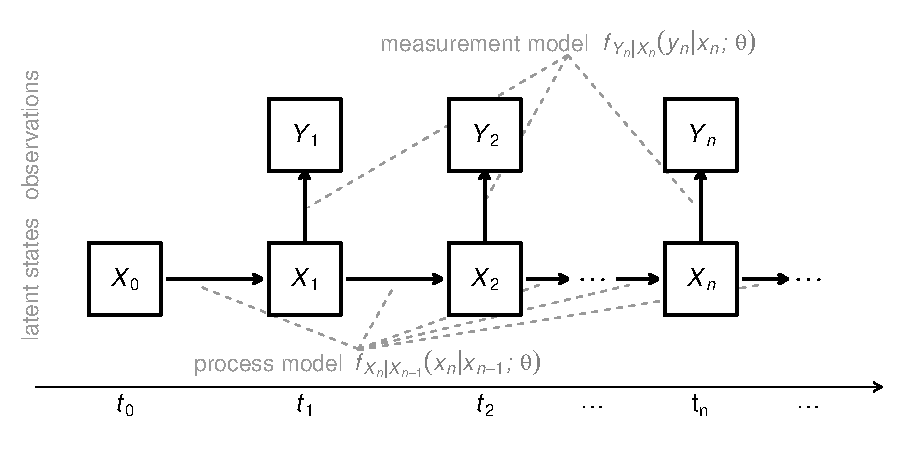
\includegraphics[width=0.75\maxwidth]{figure/pompDiagram-1} 
\end{knitrout}
\caption{\label{fig:pompDiagram}A flow diagram representing an arbitrary POMP model. Modified figure from SBIED course (King, Ionides).}
\end{figure}

Each of the SSMs considered in this thesis are POMP models.

\end{frame}

\begin{frame}{Other synonyms and definitions}
  Other common terms that are sometimes used as synonyms are used for special cases 
  \begin{block}{Mechanistic Model}
    A SSM (or POMP) where the evolution of latent variables is dictated by equations that mimic real-world mechanisms. 
  \end{block}
  
  \begin{block}{Hidden Markov Model (HMM)}
    A SSM (or POMP) where the latent variables $\bm{X}_n$ take values in a discrete and finite space.
  \end{block}

I chose SSM for the title as it is the terminology that potential collaborators are most familiar with.

\end{frame}

\begin{frame}{Remaining Chapters and Outline}
  \begin{itemize}
    \item \alert{Chapter~2:} Inference for $\mathrm{ARMA}$ models.
      \begin{itemize}
        \item $\mathrm{ARMA}$ models are a special type of linear Gaussian SSMs, and are an important part of modern science (In review). 
      \end{itemize}
    \item \alert{Chapter~3:} Mechanistic models for modeling cholera \citep{wheeler24}.
      \begin{itemize}
        \item This case study discusses the strengths and weaknesses of using mechanistic models to inform government policy, using a retrospective analysis of the 2010-2019 cholera outbreak in Haiti.
      \end{itemize}
    \item \alert{Chapter~4:} The marginalized panel iterated filter (MPIF) algorithm.
    \begin{itemize}
      \item A new inference algorithm is proposed for a large collections of related POMP models, called PanelPOMPs, and theory for existing algorithms for these models is also presented.
    \end{itemize}
    \item \alert{Chapter~5:} Summary and future directions.
  \end{itemize}
\end{frame}

\end{document}
%EoF


\documentclass[aspectratio=169]{beamer}\usepackage[]{graphicx}\usepackage[]{xcolor}
% maxwidth is the original width if it is less than linewidth
% otherwise use linewidth (to make sure the graphics do not exceed the margin)
\makeatletter
\def\maxwidth{ %
  \ifdim\Gin@nat@width>\linewidth
    \linewidth
  \else
    \Gin@nat@width
  \fi
}
\makeatother

\definecolor{fgcolor}{rgb}{0.345, 0.345, 0.345}
\newcommand{\hlnum}[1]{\textcolor[rgb]{0.686,0.059,0.569}{#1}}%
\newcommand{\hlsng}[1]{\textcolor[rgb]{0.192,0.494,0.8}{#1}}%
\newcommand{\hlcom}[1]{\textcolor[rgb]{0.678,0.584,0.686}{\textit{#1}}}%
\newcommand{\hlopt}[1]{\textcolor[rgb]{0,0,0}{#1}}%
\newcommand{\hldef}[1]{\textcolor[rgb]{0.345,0.345,0.345}{#1}}%
\newcommand{\hlkwa}[1]{\textcolor[rgb]{0.161,0.373,0.58}{\textbf{#1}}}%
\newcommand{\hlkwb}[1]{\textcolor[rgb]{0.69,0.353,0.396}{#1}}%
\newcommand{\hlkwc}[1]{\textcolor[rgb]{0.333,0.667,0.333}{#1}}%
\newcommand{\hlkwd}[1]{\textcolor[rgb]{0.737,0.353,0.396}{\textbf{#1}}}%
\let\hlipl\hlkwb

\usepackage{framed}
\makeatletter
\newenvironment{kframe}{%
 \def\at@end@of@kframe{}%
 \ifinner\ifhmode%
  \def\at@end@of@kframe{\end{minipage}}%
  \begin{minipage}{\columnwidth}%
 \fi\fi%
 \def\FrameCommand##1{\hskip\@totalleftmargin \hskip-\fboxsep
 \colorbox{shadecolor}{##1}\hskip-\fboxsep
     % There is no \\@totalrightmargin, so:
     \hskip-\linewidth \hskip-\@totalleftmargin \hskip\columnwidth}%
 \MakeFramed {\advance\hsize-\width
   \@totalleftmargin\z@ \linewidth\hsize
   \@setminipage}}%
 {\par\unskip\endMakeFramed%
 \at@end@of@kframe}
\makeatother

\definecolor{shadecolor}{rgb}{.97, .97, .97}
\definecolor{messagecolor}{rgb}{0, 0, 0}
\definecolor{warningcolor}{rgb}{1, 0, 1}
\definecolor{errorcolor}{rgb}{1, 0, 0}
\newenvironment{knitrout}{}{} % an empty environment to be redefined in TeX

\usepackage{alltt}
\usetheme{gotham}

	\usepackage{standalone}
	\usepackage{tikz}
	\usepackage{pgfplots}
	\usepackage{tabularray} % Typeset tabulars and arrays (contains equivalent of longtable, booktabs and dcolumn at least)
		\UseTblrLibrary{booktabs} % to load extra commands from booktabs
	\usepackage{changepage}
	\usepackage{minted}
		\definecolor{codeback}{rgb}{0.90,0.91,0.92}
		\definecolor{codebackdark}{rgb}{0.10,0.11,0.12}

	\newcommand{\famName}[1]{\textsc{#1}}
	\newcommand{\themename}{\textbf{\textsc{Gotham}}}

\begin{knitrout}
\definecolor{shadecolor}{rgb}{0.969, 0.969, 0.969}\color{fgcolor}\begin{kframe}
\begin{alltt}
\hlkwd{library}\hldef{(arima2)}
\end{alltt}


{\ttfamily\noindent\itshape\color{messagecolor}{\#\# \\\#\# Attaching package: 'arima2'}}

{\ttfamily\noindent\itshape\color{messagecolor}{\#\# The following object is masked from 'package:stats':\\\#\# \\\#\# \ \ \ \ arima}}\begin{alltt}
\hlkwd{library}\hldef{(tidyverse)}
\end{alltt}


{\ttfamily\noindent\itshape\color{messagecolor}{\#\# -- Attaching core tidyverse packages --------------------------------------------------- tidyverse 2.0.0 --\\\#\# v dplyr \ \ \ \ 1.1.4 \ \ \ \ v readr \ \ \ \ 2.1.5\\\#\# v forcats \ \ 1.0.0 \ \ \ \ v stringr \ \ 1.5.1\\\#\# v ggplot2 \ \ 3.5.2 \ \ \ \ v tibble \ \ \ 3.2.1\\\#\# v lubridate 1.9.4 \ \ \ \ v tidyr \ \ \ \ 1.3.1\\\#\# v purrr \ \ \ \ 1.0.4}}

{\ttfamily\noindent\itshape\color{messagecolor}{\#\# -- Conflicts --------------------------------------------------------------------- tidyverse\_conflicts() --\\\#\# x dplyr::filter() masks stats::filter()\\\#\# x dplyr::lag() \ \ \ masks stats::lag()\\\#\# i Use the conflicted package (<http://conflicted.r-lib.org/>) to force all conflicts to become errors}}\begin{alltt}
\hlkwd{library}\hldef{(latex2exp)}
\hldef{root} \hlkwb{<-} \hlsng{""}
\end{alltt}
\end{kframe}
\end{knitrout}

\IfFileExists{upquote.sty}{\usepackage{upquote}}{}
\begin{document}

\section{Likelihood Maximization for ARMA models}

\begin{frame}{Auto-regressive moving average (ARMA) models}
  ARMA models are the most frequently used approach to modeling time series data.
  ARMA models are as foundational to time series analysis as linear models are to regression analysis, and they are often used in conjunction for regression with ARMA errors.
  
  \begin{block}{ARMA model definition}
    A time series $Y_{1:N}$ is called ARMA$(p, q)$ if it is (weakly) stationary and
    \begin{equation}
    Y_n = \phi_1Y_{n - 1} + \cdots + \phi_pY_{n - p} + w_n + \MApar_1w_{n-1} + \ldots + \MApar_qw_{n - q},\label{eq:arma}
    \end{equation}
    with $\{w_n; n = 0, \pm1, \pm2, \ldots\}$ denoting a mean zero white noise (WN) processes with variance $\sigma_w^2 > 0$, and $\phi_p \neq 0$, $\MApar_q \neq 0$.
  \end{block}
  
  We refer to the positive integers $p$ and $q$ of Eq.~\myeqref{eq:arma} as the autoregressive (AR) and moving average (MA) orders, respectively.
\end{frame}

\begin{frame}[allowframebreaks]{State space formulation}
  For practitioners, ARMA models do not appear to be SSMs.
  However, inference methodology treats ARMA models as \emph{non-mechanistic} SMMs. Let $r = \max(p, q+1)$, and we now define
  \begin{equation*}
    X_n = \begin{pmatrix}
  Y_n \\
  \phi_2 Y_{n - 1} + \ldots + \phi_r Y_{n - r + 1} + \MApar_{1}w_{n} + \ldots + \MApar_{r - 1}w_{n - r + 2} \\
    \phi_3 Y_{n - 1} + \ldots + \phi_r Y_{n - r + 2} + \MApar_{2}w_{n} + \ldots + \MApar_{r - 1}w_{n - r + 3} \\
    \vdots \\
    \phi_r Y_{n - 1} + \MApar_{r - 1}w_n
  \end{pmatrix} \in \R^r
  \end{equation*}
  \begin{equation*}
  T = \begin{pmatrix}
\phi_1 & 1 & 0 & \ldots & 0 \\
\phi_2 & 0 & 1 & \ldots & 0 \\
\vdots & \vdots & & \ddots & \\
\phi_{r-1} & 0 & \ldots &  & 1 \\
\phi_r & 0 & \ldots & & 0
\end{pmatrix} \in \R^{r \times r}, \quad\quad
Q = \begin{pmatrix}
  1 \\ \MApar_1 \\ \vdots \\ \MApar_{r - 1} \in \R^r
\end{pmatrix}
  \end{equation*}

We can then recover the ARMA model using the following state space formulation:
\begin{align*}
  X_n &= TX_{n - 1} + Qw_n \\
  Y_n &= \begin{pmatrix} 1 & 0 & \ldots & 0\end{pmatrix} X_n
\end{align*}

This results in a linear-Gaussian SSM, and the likelihood function $\mathcal{L}(\paramVec)$ can be evaluated exactly using the Kalman filter \citep{kalman60}.
\begin{itemize}
  \item The likelihood can be maximized by combining this with a numeric optimizer \citep{gardner1980}.
\end{itemize}

This approach has been the standard method for fitting ARIMA models since the early 2000's due to modern computing capabilities \citep{ripley2002}. 

\end{frame}

\begin{frame}{Optimization Shortcomings}
This existing approach frequently results in sub-optimal parameter estimates.
To demonstrate this, we fit an ARMA$(2, 2)$ and an ARMA$(2, 1)$ model to data generated from an ARMA$(2, 2)$ model. 
The ARMA$(2, 1)$ is formally a special case of an ARMA$(2, 2)$ model, with $\MApar_2 = 0$. 

In \code{R}, we draw a single instance from Model class 2: $y^*_{1:100} \sim \mathrm{ARMA}(2, 2)$ with: 
\begin{itemize}
  \item $(\phi_1, \phi_2, \MApar_1, \MApar_2) = (0.2, -0.1, 0.4, 0.2)$
  \item $w_n \overset{\text{iid}}{\sim} N(0, 1)$. 
  \item Intercept $\mu = 13$ so that $E[Y_n] \neq 0$.
\end{itemize}



\end{frame}

\begin{frame}{Fitting ARMA models}
\setbeamercovered{transparent}

The \citet{gardner1980} is the standard method for fitting ARMA model parameters. It is implemented in the base \code{stats} package in R, as well as the \code{statsmodels} module in Python.

% Now we fit both both classes of models: $\mathrm{ARMA}(2, 1)$ and $\mathrm{ARMA}(2, 2)$: 
\begin{knitrout}
\definecolor{shadecolor}{rgb}{0.969, 0.969, 0.969}\color{fgcolor}\begin{kframe}
\begin{alltt}
\hldef{mod1} \hlkwb{<-} \hldef{stats}\hlopt{::}\hlkwd{arima}\hldef{(y,} \hlkwc{order} \hldef{=} \hlkwd{c}\hldef{(}\hlnum{2}\hldef{,} \hlnum{0}\hldef{,} \hlnum{1}\hldef{))}

\hldef{mod2} \hlkwb{<-} \hldef{stats}\hlopt{::}\hlkwd{arima}\hldef{(y,} \hlkwc{order} \hldef{=} \hlkwd{c}\hldef{(}\hlnum{2}\hldef{,} \hlnum{0}\hldef{,} \hlnum{2}\hldef{))}
\end{alltt}
\end{kframe}
\end{knitrout}

\pause 
The likelihood of \code{mod1} is -141.2, and the likelihood of \code{mod2} is -144.3. The \alert{smaller} model has a log-likelihood that is 3.1 units \alert{higher} than the larger model, which is mathematically impossible under proper optimization. 
\end{frame}

\begin{frame}{Convergence to local optima}
  The difficulty is that the likelihood surface is often multimodal, and the existing procedure runs the risk of converging to a local solution \citep{ripley2002}.


  

\begin{figure}[ht]
\begin{knitrout}
\definecolor{shadecolor}{rgb}{0.969, 0.969, 0.969}\color{fgcolor}
\includegraphics[width=0.9\maxwidth]{figure/mutliMode-fig-1} 
\end{knitrout}
\caption{\label{fig:multiMode}The profile log-likelihood of data simulated from four distinct MA(1) models. The dashed, red line indicates the true value of $\MApar_1$; the short-dashed blue line is the CSS-initialization. The solid black line correspond to the estimate $\hat{\MApar}_1$ using \code{stats:arima}.}
\end{figure}

\end{frame}

\begin{frame}{Multiple parameter initializations}
\setbeamercovered{transparent}
  In other contexts with multi-model loss functions, the optimization is often repeated using multiple initializations. 
  However, I have seen \alert{no instances} of this for ARIMA models. There are a few challenges: 
  \begin{itemize}
    \item Most users don't know about the possibility of converging to local solutions. 
    \item Their are complex constraints of possible initialization. 
    \begin{itemize}
      \item Constraints are on the roots of polynomials formed by model parameters, not directly on parameters themselves.
    \end{itemize}
  \end{itemize}
  \pause
  The roots of the polynomials $\Phi(x) = 1 - \phi_1 x - \phi_2x^2 - \ldots - \phi_px^p$ and $\Psi(x) = 1 + \MApar_1 x + \MApar_2x^2 + \ldots + \MApar_qx^q$ must lie outside the complex unit circle.
\end{frame}

\begin{frame}
  For parameters to be real, the roots need to be sampled as real or conjugate pairs. We cannot sample all roots as conjugate pairs (or real), as this would result in specific parameters being all one sign. Our approach for each root is the following:
  \begin{itemize}
    \item Sample inverted-root magnitudes uniformly $U(\gamma, 1-\gamma)$.
    \item With probability $p = \sqrt{1/2}$, sample inverted-root pairs as real.
    \begin{itemize}
      \item If real, assign the same sign with probability $p$.
      \item If complex, sample angle from $U(0, \pi)$, and use to assign conjugate pairs of inverted-roots.
    \end{itemize}
    \item With roots sampled, calculate corresponding coefficients and perform optimization routine.
    \item Repeat until convergence.
  \end{itemize}
\end{frame}

\begin{frame}{Revisiting toy example}
\setbeamercovered{transparent}

Now we'll fit the exact same models using the \code{arima2} package:



\begin{knitrout}
\definecolor{shadecolor}{rgb}{0.969, 0.969, 0.969}\color{fgcolor}\begin{kframe}
\begin{alltt}
\hldef{mod1v2} \hlkwb{<-} \hldef{arima2}\hlopt{::}\hlkwd{arima}\hldef{(y,} \hlkwc{order} \hldef{=} \hlkwd{c}\hldef{(}\hlnum{2}\hldef{,} \hlnum{0}\hldef{,} \hlnum{1}\hldef{))}

\hldef{mod2v2} \hlkwb{<-} \hldef{arima2}\hlopt{::}\hlkwd{arima}\hldef{(y,} \hlkwc{order} \hldef{=} \hlkwd{c}\hldef{(}\hlnum{2}\hldef{,} \hlnum{0}\hldef{,} \hlnum{2}\hldef{))}
\end{alltt}
\end{kframe}
\end{knitrout}

With this new algorithm and software, the likelihood of \code{mod1v2} is -141.2, and the likelihood of \code{mod2v2} is -141.2.

\pause
The likelihood of the smaller model was unchanged, but the larger model had an increase in log-likelihood of 3.1. The likelihoods of the nested models are now \alert{consistent}.
\end{frame}

\begin{frame}{Summary}
\setbeamercovered{transparent}
ARMA models are not necessarily state-of-the art statistical models. Why does this project matter?
  \begin{itemize}
    \item ARMA models are among the most frequently used approaches in all of statistics, so even small improvements are worth the effort.\pause
    \item Software that claims to maximize model likelihoods fails to do so in a large number of cases ($>20\%$).\pause
    \item ARMA models are often used in conjunction with linear regression. Likelihood ratio tests are common for testing the inclusion / significance of regression parameters.\pause
    \begin{itemize}
      \item Typical improvements in log-likelihood in the range $(0.22, 1.46)$. This shortcoming in one or both model is large enough to change the outcome of these tests.\pause
    \end{itemize}
    \item Even if outcomes are unchanged, confidence that software / algorithms will reliably do what you expect is important. 
  \end{itemize}
\end{frame}

\end{document}
%EoF


\documentclass[aspectratio=169]{beamer}\usepackage[]{graphicx}\usepackage[]{xcolor}
% maxwidth is the original width if it is less than linewidth
% otherwise use linewidth (to make sure the graphics do not exceed the margin)
\makeatletter
\def\maxwidth{ %
  \ifdim\Gin@nat@width>\linewidth
    \linewidth
  \else
    \Gin@nat@width
  \fi
}
\makeatother

\definecolor{fgcolor}{rgb}{0.345, 0.345, 0.345}
\newcommand{\hlnum}[1]{\textcolor[rgb]{0.686,0.059,0.569}{#1}}%
\newcommand{\hlsng}[1]{\textcolor[rgb]{0.192,0.494,0.8}{#1}}%
\newcommand{\hlcom}[1]{\textcolor[rgb]{0.678,0.584,0.686}{\textit{#1}}}%
\newcommand{\hlopt}[1]{\textcolor[rgb]{0,0,0}{#1}}%
\newcommand{\hldef}[1]{\textcolor[rgb]{0.345,0.345,0.345}{#1}}%
\newcommand{\hlkwa}[1]{\textcolor[rgb]{0.161,0.373,0.58}{\textbf{#1}}}%
\newcommand{\hlkwb}[1]{\textcolor[rgb]{0.69,0.353,0.396}{#1}}%
\newcommand{\hlkwc}[1]{\textcolor[rgb]{0.333,0.667,0.333}{#1}}%
\newcommand{\hlkwd}[1]{\textcolor[rgb]{0.737,0.353,0.396}{\textbf{#1}}}%
\let\hlipl\hlkwb

\usepackage{framed}
\makeatletter
\newenvironment{kframe}{%
 \def\at@end@of@kframe{}%
 \ifinner\ifhmode%
  \def\at@end@of@kframe{\end{minipage}}%
  \begin{minipage}{\columnwidth}%
 \fi\fi%
 \def\FrameCommand##1{\hskip\@totalleftmargin \hskip-\fboxsep
 \colorbox{shadecolor}{##1}\hskip-\fboxsep
     % There is no \\@totalrightmargin, so:
     \hskip-\linewidth \hskip-\@totalleftmargin \hskip\columnwidth}%
 \MakeFramed {\advance\hsize-\width
   \@totalleftmargin\z@ \linewidth\hsize
   \@setminipage}}%
 {\par\unskip\endMakeFramed%
 \at@end@of@kframe}
\makeatother

\definecolor{shadecolor}{rgb}{.97, .97, .97}
\definecolor{messagecolor}{rgb}{0, 0, 0}
\definecolor{warningcolor}{rgb}{1, 0, 1}
\definecolor{errorcolor}{rgb}{1, 0, 0}
\newenvironment{knitrout}{}{} % an empty environment to be redefined in TeX

\usepackage{alltt}
\usetheme{gotham}

	\usepackage{standalone}
	\usepackage{tikz}
	\usepackage{pgfplots}
	\usepackage{tabularray} % Typeset tabulars and arrays (contains equivalent of longtable, booktabs and dcolumn at least)
		\UseTblrLibrary{booktabs} % to load extra commands from booktabs
	\usepackage{changepage}
	\usepackage{minted}
		\definecolor{codeback}{rgb}{0.90,0.91,0.92}
		\definecolor{codebackdark}{rgb}{0.10,0.11,0.12}

	\newcommand{\famName}[1]{\textsc{#1}}
	\newcommand{\themename}{\textbf{\textsc{Gotham}}}
\IfFileExists{upquote.sty}{\usepackage{upquote}}{}
\begin{document}

\section{Informing Policy via Dynamic Models: Cholera in Haiti}

\begin{frame}{Introduction}
  \setbeamercovered{transparent}
  One of the most scientifically interesting types of SSMs are \emph{mechanistic models}.
  
  \begin{itemize}
    \item Used when we have some understanding of how a dynamic system evolves over time. 
    \item Useful in modern science, and have some advantages over machine learning models \citep{baker18,hogg24}:
    \begin{itemize}
      \item Accounting for known (but unobserved) features can improve model performance. 
      \item More intepretable. 
      \item Facilitates predictions of interventions and other counter-factuals. 
    \end{itemize}
  \end{itemize}
  \pause
  In this chapter, I demonstrate these capabilities by fitting mechanistic models to the 2010-2019 cholera outbreak in Haiti. 
\end{frame}

\begin{frame}{Cholera in Haiti}
 \begin{tabular}{cl}  
         \begin{tabular}{c}
           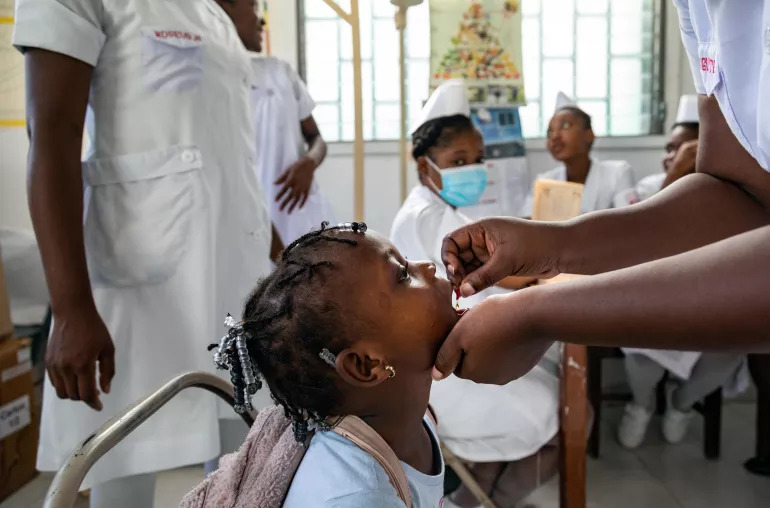
\includegraphics[height=4.3cm, width=5.5cm]{haiti/vaccination.jpeg}
           \end{tabular}
           & \begin{tabular}{l}
             \parbox{0.5\linewidth}{%  change the parbox width as appropiate
             \begin{itemize}
              \item Haiti experienced a cholera outbreak following the devastating 2010 earthquake. 
              \item From 2010-2019, more than \alert{800,000} recorded cases, making it one of the largest recorded outbreaks.
              \item Oral cholera vaccination (OCV) is available, but in limited supply.
              \item Image credit: \citet{unicef22}.
             \end{itemize}
    }
         \end{tabular}  \\
\end{tabular}
\end{frame}

\begin{frame}{Proposing interventions}
% At the time, there was interest in whether or not vaccinations would be a viable approach to eradicate cholera from Haiti.

A group of top researchers built three mechanistic models to estimate the potential impacts of various vaccination strategies \citep{lee20}.

\begin{itemize}
  \item 
\end{itemize}

\end{frame}

\end{document}
%EoF


\documentclass[aspectratio=169]{beamer}\usepackage[]{graphicx}\usepackage[]{xcolor}
% maxwidth is the original width if it is less than linewidth
% otherwise use linewidth (to make sure the graphics do not exceed the margin)
\makeatletter
\def\maxwidth{ %
  \ifdim\Gin@nat@width>\linewidth
    \linewidth
  \else
    \Gin@nat@width
  \fi
}
\makeatother

\definecolor{fgcolor}{rgb}{0.345, 0.345, 0.345}
\newcommand{\hlnum}[1]{\textcolor[rgb]{0.686,0.059,0.569}{#1}}%
\newcommand{\hlsng}[1]{\textcolor[rgb]{0.192,0.494,0.8}{#1}}%
\newcommand{\hlcom}[1]{\textcolor[rgb]{0.678,0.584,0.686}{\textit{#1}}}%
\newcommand{\hlopt}[1]{\textcolor[rgb]{0,0,0}{#1}}%
\newcommand{\hldef}[1]{\textcolor[rgb]{0.345,0.345,0.345}{#1}}%
\newcommand{\hlkwa}[1]{\textcolor[rgb]{0.161,0.373,0.58}{\textbf{#1}}}%
\newcommand{\hlkwb}[1]{\textcolor[rgb]{0.69,0.353,0.396}{#1}}%
\newcommand{\hlkwc}[1]{\textcolor[rgb]{0.333,0.667,0.333}{#1}}%
\newcommand{\hlkwd}[1]{\textcolor[rgb]{0.737,0.353,0.396}{\textbf{#1}}}%
\let\hlipl\hlkwb

\usepackage{framed}
\makeatletter
\newenvironment{kframe}{%
 \def\at@end@of@kframe{}%
 \ifinner\ifhmode%
  \def\at@end@of@kframe{\end{minipage}}%
  \begin{minipage}{\columnwidth}%
 \fi\fi%
 \def\FrameCommand##1{\hskip\@totalleftmargin \hskip-\fboxsep
 \colorbox{shadecolor}{##1}\hskip-\fboxsep
     % There is no \\@totalrightmargin, so:
     \hskip-\linewidth \hskip-\@totalleftmargin \hskip\columnwidth}%
 \MakeFramed {\advance\hsize-\width
   \@totalleftmargin\z@ \linewidth\hsize
   \@setminipage}}%
 {\par\unskip\endMakeFramed%
 \at@end@of@kframe}
\makeatother

\definecolor{shadecolor}{rgb}{.97, .97, .97}
\definecolor{messagecolor}{rgb}{0, 0, 0}
\definecolor{warningcolor}{rgb}{1, 0, 1}
\definecolor{errorcolor}{rgb}{1, 0, 0}
\newenvironment{knitrout}{}{} % an empty environment to be redefined in TeX

\usepackage{alltt}
\usetheme{gotham}

	\usepackage{standalone}
	\usepackage{tikz}
	\usepackage{pgfplots}
	\usepackage{tabularray} % Typeset tabulars and arrays (contains equivalent of longtable, booktabs and dcolumn at least)
		\UseTblrLibrary{booktabs} % to load extra commands from booktabs
	\usepackage{changepage}
	\usepackage{minted}
		\definecolor{codeback}{rgb}{0.90,0.91,0.92}
		\definecolor{codebackdark}{rgb}{0.10,0.11,0.12}

	\newcommand{\famName}[1]{\textsc{#1}}
	\newcommand{\themename}{\textbf{\textsc{Gotham}}}



\IfFileExists{upquote.sty}{\usepackage{upquote}}{}
\begin{document}

\section{The Marginalized Panel Iterated Filter (MPIF)}

\begin{frame}{Motivation}
Often we have a collection of related time series called, called \emph{panel data}.
We want to make inference using the entire collection, not just on each time series.

Examples:
  \begin{itemize}
    \item Model for disease outbreaks of the same disease, different locations (hospitals / cities) \citep{lee20}.
    \item Experiments / observational studies on ecological populations \citep{searle16}.
    \item Longitudinal studies using within-host dynamic models \citep{ranjeva17}.
  \end{itemize}
  
  Mechanistic models are routinely fitted to time series data but seldom to panel data, despite its widespread availability.
  
  % This suggests that the practical difficulties for existing procedures. 
\end{frame}

\begin{frame}{Panel models}
  Measurements for unit $u$ taken at times $t_{u, 1:N_u}$. Observed and latent process at these times denoted $Y_{u, n}$ and $X_{u, n}$, respectively.
  
  Each unit $u$ defines an independent POMP model, the entire collection of models is a PanelPOMP.
  
  $$
  \mathcal{L}(\paramVec; \bm{y}^*) = \int \prod_{u = 1}^U f_{X_{u, 0}}\big(x_{u, 0};\, \paramVec\big)\prod_{n = 1}^{N_u} f_{X_{u, n}|X_{u, n-1}}\big(x_{u, n}|x_{u, n-1}; \, \paramVec\big)f_{Y_{u, n}|X_{u, n}}\big(y_{u, n}|x_{u, n}; \, \paramVec\big) dx_{1:U,0:N_u}.
  $$
  
  The parameter vector $\theta$ has shared components $\phi$, and unit specific components $\psi_{1:U}$.
  $$\theta = (\phi, \psi_{1:U})$$
  
\end{frame}

\begin{frame}{The problem}

  Independent models, why not do inference independently? 

  \begin{itemize}
    \item Each model may share features (or parameters), and we want to estimate using all of the data. 
  \end{itemize}
  Common inference procedures in low dimensions rely on particle filters \citep{arulampalam02}.
  \begin{itemize}
    \item[{\color{green} $\checkmark$}] Particle filters work in low-dimensions, can be applied independently to units.
    \item[{\color{red} $X$}] Iterated filtering (IF) is an extension used to perform maximum likelihood estimation \citep{ionides15}.
    \begin{itemize}
      \item IF introduces dependence because of shared $\theta$, making it a high-dimensional problem.
    \end{itemize}
  \end{itemize}

\end{frame}

\begin{frame}{Background: Data cloning and iterated filtering}
  
  IF is a special type of Data cloning \citep{lele07}. 
  
  Denote $\pi_i(\theta)$ as the posterior distribution of the parameter vector $\theta$ after the $i$th Bayesian update, and $\mathcal{L}(\paramVec; \bm{y}^*)$ as the likelihood
\begin{align*}
\pi_1(\theta) &\propto \mathcal{L}(\paramVec; \bm{y}^*)\pi_0(\theta), \\
\pi_2(\theta) &\propto \mathcal{L}(\paramVec; \bm{y}^*)\pi_1(\theta) \propto \mathcal{L}(\paramVec; \bm{y}^*)^2\pi_0(\theta),\\
&\vdots\\
\pi_m(\theta) &\propto \mathcal{L}(\paramVec; \bm{y}^*)^m\pi_0(\theta).
\end{align*}
If we let $m\rightarrow \infty$, the effect of the initial prior distribution diminishes, and the $m$th posterior has all of its mass centered at the MLE.

\end{frame}

\begin{frame}{Iterated filtering}
\setbeamercovered{transparent}
  Loosely speaking, iterated filtering is just data cloning with the additional pieces: 
  \begin{enumerate}
    \item Likelihood cannot be evaluated exactly, it's approximated using particle filters. 
    \item At each time-step, the parameter particles are perturbed.
    \item Parameter particles reweighted using conditional log-likelihoods.
  \end{enumerate}\pause
  {\color{green} $\checkmark$} The perturbation of parameters is necessary to avoid particle depletion, a known problem with particle filters + Bayesian inference \citep{chen24}.
  
  {\color{red} $X$} The perturbations introduce a loss of information \citep{liu01}, so are decreased over the cloning iteration.
\end{frame}

\begin{frame}{PIF Theory}
  The panel iterated filter (PIF) is a type of IF, mitigating information loss \citep{breto20}. 
  It has been successfully used to estimate the MLE previously \citep[e.g.,][]{domeyer22}.
  
  \begin{theorem}[Chapter 4, Theorem 1]
    Extends theory of \citet{chen24} to panel models. Denote the output of the PIF algorithm as $\Theta_{1:J}^{(M)}$.
  Then there exists some positive sequences $\{C_M\}_{M \geq 1}$ and $\{\epsilon_M\}_{M \geq 1}$ where $\lim_{M \rightarrow \infty}\epsilon_M = 0$ such that for all $(J, M) \in \mathbb{N}^2$,
  $$
  E\bigg[\Big|\frac{1}{J}\sum_{i=1}^J \Theta_j^{(M)} - \hat{\theta}\Big|_2\bigg] \leq \frac{C_M}{\sqrt{J}} + \epsilon_M
  $$
  \end{theorem}
  
\end{frame}

\begin{frame}{Proof sketch and discussion}
  Conditions:
  \begin{itemize}
    \item On parameter space $\Theta$: Compact, corners not too ``sharp" \citep[regular compact set, Def~1 of][]{chen24}.
    \item Regularity conditions on the model (positive and finite likelihood, densities are smooth functions of $\theta$). 
    \item Conditions on the parameter perturbations (type of perturbations, and cooling schedule). 
  \end{itemize}
  Proof Sketch: 
  \begin{itemize}
    \item \citet{chen24} provides theory for convergence of IF of POMP models; we write a general PanelPOMP as a POMP model, and PIF is a special case of IF for these models. 
  \end{itemize}
\end{frame}

\begin{frame}{Iterated Filtering for panel models: a tradeoff}
  Iterated filtering is done one observation at a time. 
  In the panel setting, this means we also process one unit $u$ at a time.
  
  Ignoring perturbations, we have do \emph{unit} data cloning, iterating over $(m, u)$: 
  \begin{align}
    \pi_{m, u}(\theta) &\propto \mathcal{L}(\paramVec; y_u^*)\, \pi_{m, u-1}(\theta) = \mathcal{L}_u(\phi, \psi_u; y_u^*)\, \pi_{m, u-1}(\theta), \label{eq:PIFupdate}
  \end{align}
    Using $\pi_{0, 0}(\theta)$ as the initial prior distribution. Parameter dependence in posteriors introduced by iterating Eq.~\ref{eq:PIFupdate} over $u$.
    
    Two options of iterated filtering: 
    \begin{itemize}
      \item Perturb all parameters at each time step (IF2, high loss of information). 
      \item When using data from unit $u$, only perturb $\phi$ and $\psi_u$ (PIF, high particle depletion). 
    \end{itemize}
\end{frame}

\begin{frame}{MPIF motivation}
\setbeamercovered{transparent}
  If the previous prior $\pi_{m, u-1}(\theta)$ has parameter independence: $\pi_{m, u-1}(\theta) = f(\psi_{-u})g(\phi, \psi_{u})$, then there is no need to resample particles $\psi_{-u}$. 
  
  This would avoid the particle depletion \emph{and} loss-of-information, and motivates marginalized data cloning (repeating Eqs.~\ref{eq:margBayes}--\ref{eq:MPIFupdate}).
  
  \begin{align}
\tilde{\pi}_{m, u}(\theta) &\propto \mathcal{L}_{u}(y^*_u;\, \phi, \psi_u)\, \pi_{m, u-1}(\theta) \label{eq:margBayes}\\
\pi_{m, u}(\theta) &\propto \int \! \tilde{\pi}_{m, u}(\theta) \, d\phi \, d\psi_u \, \times \int \! \tilde{\pi}_{m, u}(\theta) \, d\psi_{-u} \label{eq:MPIFupdate}.
\end{align}\pause

Marginalization can happen in various ways. Next slide is a figure with bivariate Gaussian densities, marginalized over all parameters. 

\end{frame}

\begin{frame}{Marginalized Bayes: Guassian figure}

\begin{knitrout}
\definecolor{shadecolor}{rgb}{0.969, 0.969, 0.969}\color{fgcolor}

{\centering \includegraphics[width=\maxwidth]{figure/figDC-1} 

}


\end{knitrout}

\end{frame}

\begin{frame}{MPIF theory}

  Just as Iterated Filtering extends data cloning (perturbations + particle approximation), the MPIF algorithm extends marginalized data cloning. 

  \begin{itemize}
    \item Existing theory for IF algorithms rely heavily on the data cloning principle \cite{ionides15, chen24}.
    \item The non-linearity introduced by the marginalization step invalidates these approaches.
    % \item Existing theory for IF algorithms cannot readily be extended to MPIF, because of the non-linearity introduced by the marginalization step. 
    \item A natural first question is whether or not marginalized data cloning converges.
    \begin{itemize}
      \item Unfortunately, a few toy examples suggests not always (computationally and analytically).
    \end{itemize}
  \end{itemize}
  
\end{frame}

\begin{frame}{Marginalized data cloning: Gaussian likelihoods}
  Convergence is explored via Gaussian likelihoods.
  
  The properties of this special case is relevant to the broader class of models that is well approximated by Gaussian models, (e.g., local asymptotic normality \citep{lecam00}).
  
  \begin{theorem}[Chapter 4, Theorem 2]
    Let $\mathcal{L}_u(y_u^*; \, \phi, \psi_u)$ be the likelihood that corresponds to a Gaussian distribution with mean $(\phi^*, \psi_u^*)$ and precision $\Lambda_u^* \in \R^{2\times2}$. Under suitable conditions on the matrices $\Lambda^*_u$, then if the initial prior density is Gaussian, then the density of the $m$th iteration of Eq.~\ref{eq:MPIFupdate} converges to a point mass at the MLE $(\phi^*, \psi_1^*, \ldots, \psi^*_U)$ as $m\rightarrow \infty$.
  \end{theorem}
\end{frame}

\begin{frame}{Gaussian Theory: Proof sketch}

\begin{itemize}
  \item Gaussian priors + Gaussian likelihoods imply Gaussian posteriors.
  \item Transform data so likelihood is centered at zero.
  \item The marginalization step only modifies the covariance, setting off-diagonal terms to zero. Conditions ensure this loss of information is not too large.
  \item Diagonals of covariance shrink to zero asymptotically at rate $1/m$.
  \item Each unit-iteration updates the $\phi$ and $\psi_u$ components of $\mu_m$.
  \item $\mu_m = \big(\prod_{i = 1}^m\prod_{u = 1}^U A_{u, i}\big) \mu_0 = \big(\prod_{i = 1}^m P_m\big) \mu_0$, with $\|P_m\|_2 = 1 - \epsilon_m/m + o(1/m)$, with $\epsilon_m$ positive, bounded.
\end{itemize}

\end{frame}

\begin{frame}{Convergence with perturbations}

    \begin{theorem}[Chapter 4, Corollary 1]
    Considering the same setup as Theorem~2 (Chapter~4), if parameters are perturbed prior performing the Bayes update at each step using Gaussian additive noise with mean $0$ and covariance $\sigma^2_m\Sigma_0$, then if $\sigma_m^2 = o(1/m)$, then the algorithm still converges to the MLE as $m\rightarrow \infty$. 
  \end{theorem}
  
  \begin{itemize}
    \item Useful heuristic: a more dispersed prior typically results in a posterior distribution that more closely resembles the likelihood function.
    \item Adding Gaussian noise at each step results in larger updates towards to MLE at each step.
    \item Heuristically, convergence of unperturbed case implies convergence of perturbed case, if perturbation variance decreases to zero.
  \end{itemize}

\end{frame}

\begin{frame}{The MPIF advantage: improved particle representation}

  One perspective is that the marginalization adds a small amount of bias in each intermediate posterior distribution.
  
  \begin{itemize}
    \item Theorem~2 (Chapter 4) gives formal conditions where the bias at each step is small enough that the combined iterations still converge to the MLE (no bias).
    \item The advantage of MPIF, however, is improved particle representations. In this case, MPIF may still be preferable even if there is bias in final estimate.
  \end{itemize}
  
\end{frame}

\begin{frame}{Bias-Variance tradeoff}
  
\begin{knitrout}
\definecolor{shadecolor}{rgb}{0.969, 0.969, 0.969}\color{fgcolor}

{\centering \includegraphics[width=0.65\maxwidth]{figure/unnamed-chunk-1-1} 

}


\end{knitrout}
  
\end{frame}

\begin{frame}{Gompertz population model: high-dimensional space}

The MPIF algorithm is demonstrated on data simulated from a stochastic population model. We have $U$ ranging from $5--2500$, and $N_u = N \in \{20, 50, 100\}$.
\begin{itemize}
  \item $X_{u, n+1} = K^{1- \exp{r_u}}_u \epsilon_{u, n}$, $\epsilon_{u, n} \sim N(0, \sigma^2_u)$. 
  \item $Y_{u, n} | X_{u, n} \sim N\big(\log X_{u, n}, \tau^2_u\big)$
  \item Fix $K_u = 1$, $X_{u, 0} = 1$. Estimate $\sigma_u^2 = \sigma^2 = 0.01$, $r_u = r = 0.1$, and $\tau_u^2 = 0.01$ for all $u$.  
\end{itemize}

This is log-linear Gaussian, so exact likelihood can be computed \citep{kalman60}. Parameter choices match \citet{breto20}. 

\end{frame}

\begin{frame}


\begin{knitrout}
\definecolor{shadecolor}{rgb}{0.969, 0.969, 0.969}\color{fgcolor}

{\centering \includegraphics[width=\maxwidth]{figure/gompFig1-1} 

}


\end{knitrout}
\end{frame}

\begin{frame}{Discussion}
  \begin{itemize}
    \item In all tested models, the MPIF algorithm outperforms PIF, especially as the number of units $U$ is large, and number of unit-specific parameters is large.
    \item Even poor performing replicates of MPIF often outperform PIF, despite having weaker theoretical guarantees.
    \item Improved performance is a result of reduced particle depletion.
    \item Stronger theory for MPIF is available in some special cases, each covered by Theorem~1 of Chapter~4:
    \begin{itemize}
      \item No shared parameters: there is no parameter dependence, and the algorithm is equivalent to performing IF2 independently to each model. 
      \item No unit-specific parameters: the algorithm is the same as PIF, as resampling unit-specific parameters is not needed.
    \end{itemize}
  \end{itemize}
\end{frame}

\end{document}
%EoF


\documentclass[aspectratio=169]{beamer}\usepackage[]{graphicx}\usepackage[]{xcolor}
% maxwidth is the original width if it is less than linewidth
% otherwise use linewidth (to make sure the graphics do not exceed the margin)
\makeatletter
\def\maxwidth{ %
  \ifdim\Gin@nat@width>\linewidth
    \linewidth
  \else
    \Gin@nat@width
  \fi
}
\makeatother

\definecolor{fgcolor}{rgb}{0.345, 0.345, 0.345}
\newcommand{\hlnum}[1]{\textcolor[rgb]{0.686,0.059,0.569}{#1}}%
\newcommand{\hlsng}[1]{\textcolor[rgb]{0.192,0.494,0.8}{#1}}%
\newcommand{\hlcom}[1]{\textcolor[rgb]{0.678,0.584,0.686}{\textit{#1}}}%
\newcommand{\hlopt}[1]{\textcolor[rgb]{0,0,0}{#1}}%
\newcommand{\hldef}[1]{\textcolor[rgb]{0.345,0.345,0.345}{#1}}%
\newcommand{\hlkwa}[1]{\textcolor[rgb]{0.161,0.373,0.58}{\textbf{#1}}}%
\newcommand{\hlkwb}[1]{\textcolor[rgb]{0.69,0.353,0.396}{#1}}%
\newcommand{\hlkwc}[1]{\textcolor[rgb]{0.333,0.667,0.333}{#1}}%
\newcommand{\hlkwd}[1]{\textcolor[rgb]{0.737,0.353,0.396}{\textbf{#1}}}%
\let\hlipl\hlkwb

\usepackage{framed}
\makeatletter
\newenvironment{kframe}{%
 \def\at@end@of@kframe{}%
 \ifinner\ifhmode%
  \def\at@end@of@kframe{\end{minipage}}%
  \begin{minipage}{\columnwidth}%
 \fi\fi%
 \def\FrameCommand##1{\hskip\@totalleftmargin \hskip-\fboxsep
 \colorbox{shadecolor}{##1}\hskip-\fboxsep
     % There is no \\@totalrightmargin, so:
     \hskip-\linewidth \hskip-\@totalleftmargin \hskip\columnwidth}%
 \MakeFramed {\advance\hsize-\width
   \@totalleftmargin\z@ \linewidth\hsize
   \@setminipage}}%
 {\par\unskip\endMakeFramed%
 \at@end@of@kframe}
\makeatother

\definecolor{shadecolor}{rgb}{.97, .97, .97}
\definecolor{messagecolor}{rgb}{0, 0, 0}
\definecolor{warningcolor}{rgb}{1, 0, 1}
\definecolor{errorcolor}{rgb}{1, 0, 0}
\newenvironment{knitrout}{}{} % an empty environment to be redefined in TeX

\usepackage{alltt}
\usetheme{gotham}

   \usepackage{appendixnumberbeamer}
   \usepackage[scale=2]{ccicons}
   \newcommand{\themename}{\textbf{\textsc{Gotham}}}
\IfFileExists{upquote.sty}{\usepackage{upquote}}{}
\begin{document}

\section{Conclusion and future directions}

  \begin{frame}{Summary}
    Likelihood based inference of SSMs is a challenging task. This thesis presents novel research related to various aspects of this problem:
    \begin{itemize}
      \item Chapter~2 proposes new \alert{methodology} for ARIMA models, perhaps the most used type of SSM. It demonstrates existing algorithms fail to properly maximize likelihoods, and fixes this with limited additional computational effort. 
      \item Chapter~3 is an \alert{application} that proposes new standards for using mechanistic models to inform policy. It demonstrates some strengths and weaknesses of existing approaches, and how recent methodological advances can be used to aid this task. 
      \item Chapter~4 proposes new \alert{methodology} to help perform maximum likelihood estimation for high-dimensional panel models, and provides \alert{theory} for the proposed approach in special cases. It also extends existing theory for iterating filtering on panel models.
    \end{itemize}
  \end{frame}

  \begin{frame}{Future Directions: Chapter 2}
    The importance of ARIMA models to modern science additional developments related to this chapter may be worth the effort. Particularly well-suited for an undergraduate research project(s): 
    \begin{itemize}
      \item Building a Python library to implement the existing algorithm. 
      \item Consider stratified sampling of root initializations (i.e., sample from each quadrant rather than randomly).
      \item Develop theoretical bounds on the number of local optima, resulting in improved stopping criteria.
      \item Leveraging iterated filtering to do non-Gaussian ARMA models and/or in panel models.
    \end{itemize}
  \end{frame}
  
  \begin{frame}{Future Directions: Chapter 3}
    The lessons learned from this retrospective analysis may be relevant in other disciplines.
    Additionally, there are a number of things I learned that didn't make the final paper: 
    \begin{itemize}
      \item The importance of initialization and measurement models. These are often overlooked, but are key to fitting insightful models.
      \item Uncertainty propagation: the natural approach is perform Monte Carlo adjusted profile confidence intervals \citep{ionides17}, giving a large number of parameter values, and sample these using their likelihoods (Empirical Bayes). If dimensions are high, the Monte Carlo variance is high, so you don't get to resample many parameters this way. 
    \end{itemize}
  \end{frame}
  
  \begin{frame}{Future Directions: Chapter 4}
    The theory developed for both PIF and MPIF gives rise to a few extensions: 
    \begin{itemize}
      \item Current theory for MPIF ignores particle approximations, and is limited to Gaussian densities.
      \item Nested levels of shared and unit-specific parameters. This is particularly useful for performing inference on nested designed experiments, or designed experiments that may have global shared parameters, shared parameters for each experimental treatment, and unit-specific parameters for each experimental replicate.
    \end{itemize}
  \end{frame}
    
    \begin{frame}{Future Directions: General}
      Parameter perturbations introduced in IF result in loss-of-information. Recent work in automatic differentiation can help avoid this issue, though appears to require IF-algorithms to initialize \citep{tan24}. MPIF can be particularly useful for this algorithm in panel settings. Related to this extension: 
      \begin{itemize}
        \item Software for panel models with auto-diff (pypomp, work ongoing with other students).
        \item Using methodology to build shallow neural networks to model unknown mechanisms \citep[e.g.,][]{noordijk24}. 
      \end{itemize}
  \end{frame}

    \begin{frame}{Future Directions: Applications}
      My interest in methodology in SSMs is in part driven by my interest in the types of problems they solve. Some potential applications include: 
      \begin{itemize}
        \item Fisheries; long history of SSM, but particle filter / IF approach hasn't caught on. Interesting to know if this approach is useful in fisheries, or if there are lessons there to be learned.
        \begin{itemize}
          \item Concrete examples include: modeling disease progression in native cutthroat species, modeling reproductive dynamics of native cutthroat with stocked rainbow trouts (threatening native reproduction) \citep{rosenthal22}.
        \end{itemize}
        \item Disease progression in farms: plants and livestock \citep{skolstrup22}.
      \end{itemize}
  \end{frame}
  
  \begin{frame}{Acknowledgements}
    There are so many people that I would like to thank, impossible to thank everyone who has helped and supported me.
    
    I would like to give a special thanks to my advisor (Edward L. Ionides), dissertation committee (Aaron A. King, Kerby Shedden, Jeffery Regier), my family, classmates, and friends.
  \end{frame}

	% % FRAME
	% \begin{frame}{Summary}
	% 	Get the source of this theme and the demo presentation from
	% 
	% 	\begin{center}\url{https://gitlab.com/RomainNOEL/beamertheme-gotham}\end{center}
	% 
	% 	The theme \emph{itself} is licensed under a \href{http://creativecommons.org/licenses/by-sa/4.0/}{Creative Commons Attribution-ShareAlike 4.0 International License}.
	% 	\begin{center} \ccbysa \end{center}
	% \end{frame}

% 	% FRAME
%    \begin{standoutenv}
%    \begin{frame}[fragile]
%       The final slide using the standout style with command:
% 		\begin{verbatim}
% 			\begin{frame}[standout, plain]{Thank You !}
% 				Questions ?
% 		 	\end{frame }
% 		\end{verbatim}
% 
% 		\begin{center}
% 			Et voilà !
% 		\end{center}
%    \end{frame}
%    \end{standoutenv}
	
\end{document}



% \documentclass[aspectratio=169]{beamer}
\usetheme{gotham}

	\usepackage{standalone}
	\usepackage{tikz}
	\usepackage{pgfplots}
	\usepackage{tabularray} % Typeset tabulars and arrays (contains equivalent of longtable, booktabs and dcolumn at least)
		\UseTblrLibrary{booktabs} % to load extra commands from booktabs
	\usepackage{changepage}
	\usepackage{minted}
		\definecolor{codeback}{rgb}{0.90,0.91,0.92}
		\definecolor{codebackdark}{rgb}{0.10,0.11,0.12}

	\newcommand{\famName}[1]{\textsc{#1}}
	\newcommand{\themename}{\textbf{\textsc{Gotham}}}


\begin{document}

\section{Gotham Theme}

	% FRAME
	\begin{frame}[fragile]{Gotham package}

		The \themename{} theme is a Beamer theme with a minimal-ish visual style largely inspired by the \href{https://github.com/matze/mtheme}{\textsc{Metropolis} Beamer Theme} by Matthias \famName{Vogelgesang} (and some other Beamer themes).

		Yet, \themename{} is highly extendable and versatile.
		\bigskip

		First, enable the theme by classically loading it:

		\begin{minted}{tex}
			\documentclass{beamer}
			\usetheme{gotham}
		\end{minted}

		Then, all the customization can be performed at any moment in the presentation using:

		\begin{minted}{tex}
			\gothamset{<option>=...}
		\end{minted}
	\end{frame}


\subsection{Fonts}

	% FRAME
	\begin{frame}[fragile]{Gotham title formats}
		Note, that you have to have Mozilla's \emph{Fira Sans} font and XeTeX or LuaTeX installed to enjoy this wonderful typography.

		\begin{columns}[T,onlytextwidth]
		\column{0.49\textwidth}
			\themename{} supports 4 different title formats \mintinline{tex}|\gothamset{format frametitle=}|
			\begin{itemize}
				\item regular
				\item \MakeLowercase{Lower}
				\item \MakeUppercase{Upper}
				\item \MakeTitlecase{Title Case}
			\end{itemize}
		\column{0.49\textwidth}
			\themename{} supports 3 different title shape \mintinline{tex}|\gothamset{shape frametitle=...}|:
			\begin{itemize}
				\item regular
				\item \textsc{Small caps}
				\item \textit{italic}
			\end{itemize}
		\end{columns}

		\vspace{2em}
		They can either be set at once for every title type or individually.
	\end{frame}

	{ \gothamset{format frametitle=upper, shape frametitle=italic}
	% FRAME
	\begin{frame}{Titles: Upper and italic}
		This frame uses the title format options: \mintinline{tex}|format frametitle=upper|, \mintinline{tex}|shape frametitle=italic|.
	\end{frame}
	}

	{ \gothamset{shape frametitle=smallcaps, format frametitle=titlecase}
	% FRAME
	\begin{frame}{Titles: Small caps and titlecase}
		This frame uses the title format options: \mintinline{tex}|shape frametitle=smallcaps|, \mintinline{tex}|format frametitle=titlecase|.
		
		\begin{alertblock}{Potential Problems}
			Be aware that not every font supports small caps.
			If for example you typeset your presentation with pdfTeX and the Computer Modern Sans Serif font, every text in \mintinline{tex}{smallcaps} will be typeset with the Computer Modern Serif font instead.
			Please refer to the documentation if you consider using it.
			
			As a rule of thumb: just use it for plaintext-only titles.
		\end{alertblock}
	\end{frame}
	}

	{ \gothamset{format frametitle=lower}
	% FRAME
	\begin{frame}{Titles: LOWER and regular}
		This frame uses the title format options: \mintinline{tex}{format frametitle=lower}, \mintinline{tex}{shape frametitle=regular}.
	\end{frame}
	}


\subsection{Colors}

	{ \gothamset{background=dark}
	% FRAME
	\begin{frame}[fragile]{Presentation style via background color}
		The color mode (a.k.a. background color) can be changed using:
		\begin{minted}[bgcolor=codebackdark]{tex}
			\gothamset{background=dark | light | transparent}
		\end{minted}
	\end{frame}
	}

	% FRAME
	\begin{frame}[fragile]{Blocks}
		Three different block environments are pre-defined and may be styled with an optional background color.

		\begin{columns}[T,onlytextwidth]
		\column{0.3\textwidth}
			\begin{minted}{tex}
				\gothamset{
					block=native}
			\end{minted}

			\gothamset{block=native}
			\begin{block}{Default}
				Block content.
			\end{block}

			\begin{alertblock}{Alert}
				Block content.
			\end{alertblock}

			\begin{exampleblock}{Example}
				Block content.
			\end{exampleblock}

		\column{0.3\textwidth}

			\gothamset{block=transparent}
			\begin{minted}{tex}
				\gothamset{
					block=transparent}
			\end{minted}

			\begin{block}{Default}
				Block content.
			\end{block}

			\begin{alertblock}{Alert}
				Block content.
			\end{alertblock}

			\begin{exampleblock}{Example}
				Block content.
			\end{exampleblock}

		\column{0.3\textwidth}

			\gothamset{block=fill}
			\begin{minted}{tex}
				\gothamset{
					block=fill}
			\end{minted}

			\begin{block}{Default}
				Block content.
			\end{block}

			\begin{alertblock}{Alert}
				Block content.
			\end{alertblock}

			\begin{exampleblock}{Example}
				Block content.
			\end{exampleblock}

		\end{columns}
	\end{frame}

	{\gothamset{colorset=red}
	% FRAME
	\begin{frame}[fragile]{Color customization}
		The color theme can be used only in preamble with \mintinline{tex}|\usecolortheme{wolverine}| and without guarantees on the visual aspect.

		\themename{} offers predefined color setup at any time through \mintinline{tex}|\gothamset{colorset=red}|

		Otherwise, the colors can be changed manually using:
		\begin{minted}{tex}
			\colorlet{colorPale}{gPaleYell} % BG in light/normal mode
			\colorlet{colorDark}{gDarkBlack} % FG in light/normal mode
			\colorlet{colorA}{gDarkTeal} % frametitle, standin.out,
			\colorlet{colorAreversed}{gLightTeal} % frametitle, standin.in,
			\colorlet{colorB}{gMidGrey} % gray BG : progress bar, blocks
			\colorlet{colorC}{gDeepYellOr} % progress bar
			\colorlet{colorD}{gLightOrange} % alert
			\colorlet{colorE}{gLightGreen} % example
		\end{minted}
	\end{frame}
	}


\subsection{Inner}

	% FRAME
	\begin{frame}[fragile]{Title page}
		\themename{} offers the possibility to adapt the title page layout (printed with \mintinline{tex}|\maketitle| or \mintinline{tex}|\titlepage|).
		This can be achieved using:
		\begin{minted}{tex}
			\defbeamertemplate{title page}{your name}{your defintion}
			\gothamset{title page= your name}
		\end{minted}

		\themename{} also predefined several templates such as:
		\mintinline{tex}$gotham normal$ | \mintinline{tex}$gotham splitvert$ | \mintinline{tex}$gotham dividedpic$ | \mintinline{tex}$gotham reversed$
	\end{frame}

	% FRAME
	\begin{frame}[fragile]{Table of contents}
		\themename{} comes with the possibility to apply different styles for your table of contents (ToC) page.
		You can define your own ToC style as it follows:
		\begin{minted}{tex}
			\defbeamertemplate{toc page}{your name}{your def}
			\gothamset{tocframe template= your name}
		\end{minted}
		Then, referring to this template using the frame option \mintinline{tex}|[toc]| in your presentation:
		\begin{minted}{tex}
			\begin{frame}[toc]{Table of contents}
				\tableofcontents%[hideallsubsections]
			\end{frame }
		\end{minted}

		Or using one of the \themename{} predefined templates, such as: \mintinline{tex}$gotham simple | gotham bullet$
	\end{frame}

	% FRAME
	\begin{frame}[fragile]{Sections}
		\themename{} provides a multiple options to tune sections (respectively \mintinline{tex}|part|, \mintinline{tex}|section|, \mintinline{tex}|subsection| and \mintinline{tex}|subsubsection|).

		The section command \mintinline{tex}|\section{Elements}| from Beamer will appear very different.
		The section page will appear or disappear thanks to: \mintinline{tex}$\gothamset{sectionframe default=<on|off>}$, while its layout (when appearing) is controlled by:
		\begin{minted}{tex}
			\defbeamertemplate{part|sub|subsub|section frame}
				{your name}{your def}
			\gothamset{sectionframe template= your name}
		\end{minted}

		\themename{} predefined template are: \mintinline{tex}$gotham progressbar | gotham simple |$ \mintinline{tex}$gotham splitvert progressbar |$ \mintinline{tex}$gotham splitvert simple | gotham progressvert$
	\end{frame}

	% FRAME
	\begin{frame}[fragile]{Sections contents}
		After the section page, you can (de)activate a page with a table of contents for the section using \mintinline{tex}$\gothamset{sectiontocframe default=<on|off>}$, and its layout is controlled by:
		\begin{minted}{tex}
			\defbeamertemplate{toc subsection frame}{your name}{your def}
			\gothamset{sectionframe template= your name}
		\end{minted}

		\themename{} predefined template are: \mintinline{tex}$gotham simple | gotham bullet$
	\end{frame}

	% FRAME
	\begin{frame}[fragile, watermark]{Watermark}

		With \themename{} you can locally or globally add watermark to your slides by using:
		\begin{minted}{tex}
			\defbeamertemplate{background}{watermark/your name}{your def}
			\gothamset{watermark template= your name}
		\end{minted}

		Then, this watermark can be turned on locally using \mintinline{tex}|\begin{frame}[watermark]| or globally with \mintinline{tex}|\gothamset{watermark default= on}| .
	\end{frame}

	% FRAME
	\begin{standinenv}
	\begin{frame}[fragile]{Standin}

		\themename{} comes with 2 environments/special layouts named \mintinline{tex}|standin| and \mintinline{tex}|standout|.
		These special layouts can be used to emphasize some content or last slide\textellipsis

		This layout can be turned on using \mintinline{tex}|\begin{frame}[standin]| or using the dedicated environment (\mintinline{tex}|\begin{standinenv}\begin{frame}...\end{frame}\end{standinenv}|).

		Note that the background can also be tuned using:
		\begin{minted}{tex}
			\defbeamertemplate{background canvas}{standin/name}{your def}
			\gothamset{standin BG template= name}
		\end{minted}

	\end{frame}
	\end{standinenv}

	% FRAME
	\begin{frame}[standout, watermark]{Standout}
		Here is an example of standout (working as standin), which can be combined with a watermark.

		Another difference, apart the obvious color change is the font size and series.
	\end{frame}


\subsection{Outer}

	{\setbeamertemplate{frame footer}{My custom footer}
	% FRAME
	\begin{frame}[fragile]{Frame footer}
		\themename{} defines a custom Beamer template to add a text to the footer.
		It can be set via
		\begin{minted}{tex}
			\setbeamertemplate{frame footer}{My custom footer}
		\end{minted}

		Even after redefining (or not) your frame footer template, you can locally remove it with the frame option \mintinline{tex}|\begin{frame}[nofooter]|.
	\end{frame}
	}

	\title[your shorttitle]{Gotham}
	\date[shortdate]{\today}
	\author[your shortauthor name]{Romain NOËL}
	% FRAME
	\begin{frame}[fragile, rotateFooter]{rotateFooter}
		The default footer from \themename{}, it displays the \mintinline{tex}|shortdate|, \mintinline{tex}|shorttitle| and \mintinline{tex}|shortauthor|.
		So by filling these fields in your document setup, you will see them appear in your footer:
		\begin{minted}{tex}
			\title[your shorttitle]{Your title}
			\date[shortdate]{\today}
			\author[your shortauthor name]{John DOE}
		\end{minted}

		Since we always need some extra space on some frames that would like to overlay a bit the footer, \themename{}'s footer also offers possibility to be put locally on the side using \mintinline{tex}|\begin{frame}[rotateFooter]|, or globally with
		\begin{minted}{tex}
			\gothamset{rotateFooter default=on}
		\end{minted}
		If it has set globally, it can be deactivated locally with the frame option \mintinline{tex}|\begin{frame}[norotateFooter]|.
	\end{frame}

	\title[]{Gotham}
	\date[]{\today}
	\renewcommand{\gothamRightFiligrane}{%
		\rotatebox{90}{gotham right filigrane pattern}
	}
	% FRAME
	\begin{frame}[edging, fragile]{Edging}
		\themename{} has two hook commands, \mintinline{tex}|\gothamRightFiligrane| and \mintinline{tex}|\gothamLeftFiligrane|, that can be redefined to customize what to display in the edgings (a.k.a. filigrane, a.k.a. sidebar).
		As an example, one could do:
		\begin{minted}{tex}
			\renewcommand{\gothamRightFiligrane}{%
				\rotatebox{90}{gotham right filigrane pattern}
			}
		\end{minted}

		Then, to set if it should be displayed or not, globally
		\begin{minted}{tex}
			\gothamset{edging default=on}
		\end{minted}
		or locally with the frame option \mintinline{tex}|\begin{frame}[edging]| or \mintinline{tex}|\begin{frame}[noedging]|.
	\end{frame}

	% FRAME
	% \begin{nofootlineenv}
	\begin{frame}[fragile,noedging,nofooter]{Really wide contents}
		\begin{adjustwidth}{-2em}{-2em}
			If you want a really wide content in your frame, you can change the size of your margin (requires \mintinline{tex}|\usepackage{changepage}| in your preamble).
			You can also suppress the edging (\mintinline{tex}|[noedging]|) and footer (\mintinline{tex}|[nofooter]|) or even more radically footline (\mintinline{tex}|[nofootline]|).

			Here is an example combining them:
			\begin{minted}{tex}
				\begin{frame}[noedging,nofootline]{extended frame}
					\begin{adjustwidth}{-2em}{-2em}% 2em extra to the left and 2em for right margin.
						wide content
					\end{adjustwidth}
				\end{frame }
			\end{minted}
		\end{adjustwidth}
	\end{frame}
	% \end{nofootlineenv}

	{%
	\renewcommand{\gothamInstituteLogoSquare}[1][4ex]{%
		
\includegraphics[height=#1]{gotham-logo.pdf}
	}
	\logo{extra LOGO}
	% FRAME
	\begin{frame}[fragile]{Frametitle}
		\framesubtitle{with a subtitle}
		The frametile template brought by \themename{} is relatively classic: it supports \mintinline{tex}|\subframetitle| and frame continuation (with \mintinline{tex}|[allowframebreaks]|) through templates that can be tuned.
		Nevertheless, it the frametitle template also includes a hook for your institute logo in the top right corner, leaving the command \mintinline{tex}|\logo{}| free for your extra logos.

		So, one can have both logos using:
		\begin{minted}{tex}
			\renewcommand{\gothamInstituteLogoSquare}[1][4ex]{
				
\includegraphics[height=#1]{gotham-logo.pdf}
			}
			\logo{extra LOGO}
		\end{minted}
	\end{frame}
	}

	\author[]{Romain NOËL}
	{\gothamset{progressbar position=left, progressbar style= rounded box, progressbar advancement= brlt,  numbering= circle}
	% FRAME
	\begin{frame}[fragile]{Numbering and progressbar}

		\themename{} theme can numbering your frames in the bottom right corner using different styles.
		You can also decide to use a progression bar to indicate how much of your presentation remains.

		The setup of numbering and progression bar can be performed through:
		\begin{minted}{tex}
			\gothamset{numbering= totalframenumber, progressbar position=foot}
		\end{minted}

		Numbering available options are: \mintinline{tex}$none | framenumber | totalframenumber | appendixframenumber | pagenumber $ \mintinline{tex}$| totalpagenumber | circle$

		Progressbar position available options are: \mintinline{tex}$none | head | frametitle | foot | circlehead | left | right$
	\end{frame}
	}


\end{document}
%EoF



% 
% \appendix
% 
% 	\begin{frame}[fragile]{Backup slides}
% 		Sometimes, it is useful to add slides at the end of your presentation to refer to during audience questions.
% 
% 		The best way to do this is to include \verb|\usepackage{appendixnumberbeamer}| in your preamble and call \verb|\appendix| before your backup slides.
% 
% 		\themename{} will automatically turn off slide numbering and progress bars for slides in the appendix.
% 	\end{frame}


% \normalem
% References

  \begin{frame}[allowframebreaks]{References}
    \bibliographystyle{chicagoa}
    \bibliography{references}
  \end{frame}

\end{document}
